\documentclass{acm_proc_article-sp}
\usepackage{url}
\begin{document}
\title{How can we figure out what is inside thousands of spreadsheets?}
\numberofauthors{1}
\author{ \alignauthor Thomas Levine\\ \email{\_@thomaslevine.com} }
\date{6 March 2014}
\maketitle
\begin{abstract}
We have enough data today that we it may not be realistic to understand
all of them. In hopes of vaguely understanding these data, I have been
developing methods for exploring the contents of large collections of
weakly structured spreadsheets. We can get some feel for the contents
of these collections by assembling metadata about many spreadsheets and
run otherwise typical analyses on the data-about-data; this gives us some
understanding patterns in data publishing and a crude understanding of
the contents. I have also developed spreadsheet-specific search tools
that try to find related spreadsheets based on similarities in implicit
schema. By running crude statistics across many disparate datasets,
we can learn a lot about unweildy collections of poorly structured data.
\end{abstract}

\keywords{data management, spreadsheets, open data, search}

\section{Introduction}
These days, we have more data than we know what to do with. And by "data",
we often mean unclean, poorly documented spreadsheets. I started wondering
what was in all of these spreadsheets. Addressing my curiosity turned out
to be quite difficult, so I've found up developing various approaches to
understanding the contents of large collections of weakly structured
spreadsheets.

My initial curiosity stemmed from the release of thousands of spreadsheets
in government open data initiatives. I wanted to know what they had released
so that I may find interesting things in it.

More practically, I often am looking for data from multiple sources that I
can connect in relation to a particular topic. For example, in a project I had
data about cash flows through the United States treasury and wanted to join
them to data about the daily interest rates for United States bonds. In situations
like this, I usually need to know the name of the dataset or to ask around until
I find the name. I wanted a faster and more systematic approach to this.

\section{Typical approaches to exploring the contents of spreadsheets}
Before we discuss my spreadsheet exploration methods, let's discuss some
more ordinary methods that I see in common use today.

\subsection{Look at every spreadsheet}
As a baseline,
one approach is to look manually at every cell in many spreadsheets.
This takes a long time, but it is feasible in some situations.

\subsection{Use standard metaformats}
Many groups develop domain-specific metaformats for expressing a very specific
sort of data. For example, JSON API is a metaformat for expressing the
response of a database query on the web \cite{jsonapi}, Data Packages is a
metaformat for expressing metadata about a dataset \cite{datapackages},
and KML is a metaformat for expressing annotations of geographic maps.\cite{kml}

Agreement on format and metaformat makes it faster and easier to inspect
individual files. On the other hand, it does not alleviate the
need to acquire lots of different files and to at least glance at them.
We spend less time manually inspecting each dataset, but we must still
manually inspect lots of dataset.

The same sort of thing happens when data publishers provide graphs of
each individual dataset. When we provide some graphs of a dataset
rather than simply the standard data file, we are trying to make it easier for
people to understand that particular dataset, rather than trying to focus
them on a particular subset of datasets.

\subsection{Provide good metadata} \label{guidelines}
Data may be easier to find if we catalog our data well and adhere to
certain data quality standards. With this reasoning,
many "open data" guidelines provide direction as to how a person
or organization with lots of datasets might allow other people
to use them.
\cite{open-data-census,fivestars,sunlight,sebastopol,odi}

At a basic level, these guidelines suggest that data should
be available on the internet and under a free license; at the other
end of the spectrum, guidelines suggest that data be in standard
formats accompanied with particular metadata.

Datasets can be a joy to work with when these data quality guidelines
are followed, but this requires much upfront work by the publishers
of the data.

\subsection{Asking people}
In practice, I find that people learn what's in a spreadsheet through word
of mouth, even if the data are already published on the internet in standard
formats with good metadata.

Amanda Hickman teaches journalism and keeps a list of data sources for her
students. \cite{amanda}

There entire conferences about the contents of newly released datasets,
such as the annual meeting of the Association of Public Data Users.\cite{apdu}

The Open Knowledge Foundation \cite{open-data-census}
and Code for America \cite{open-data-census-us}
even conducted data censuses to determine which governments were
releasing what data publically on the internet.
In each case, volunteers searched the internet and talked to
government employees in order to determine whether each dataset was
available and to collect certain information about each dataset.

\section{How I acquire lots of spreadsheets} \label{acquire}
In order to explore methods for examining thousands of spreadsheets,
I needed to find spreadsheets that I could explore.

Many governments and other large organizations publish spreadsheets on
data catalog websites.
Data catalogs make it kind of easy to get a bunch of spreadsheets all together.
The basic approach is this.

\begin{enumerate}
\item Download a list of all of the dataset identifiers that are present in the data catalog.
\item Download the metadata document about each dataset.
\item Download data files about each dataset.
\end{enumerate}

I've implemented this for the following data catalog softwares.

\begin{itemize}
\item Socrata Open Data Portal
\item Common Knowledge Archive Network (CKAN)
\item OpenDataSoft
\end{itemize}

This allows me to get all of the data from most of the open data catalogs I know about.

After I've downloaded spreadsheets and their metadata,
I often assemble them into a spreadsheet about spreadsheets. \cite{data-driven}
In this super-spreadsheet, each record corresponds to a full
sub-spreadsheet; you could say that I am collecting features or statistics
about each spreadsheet.

\section{Crude statistics about spreadsheets}
My first approach was involved running rather crude analyses on this
interesting dataset-about-datasets that I had assembled.

\subsection{How many datasets}
I started out by simply counting how many datasets each catalog website had.

\begin{figure}
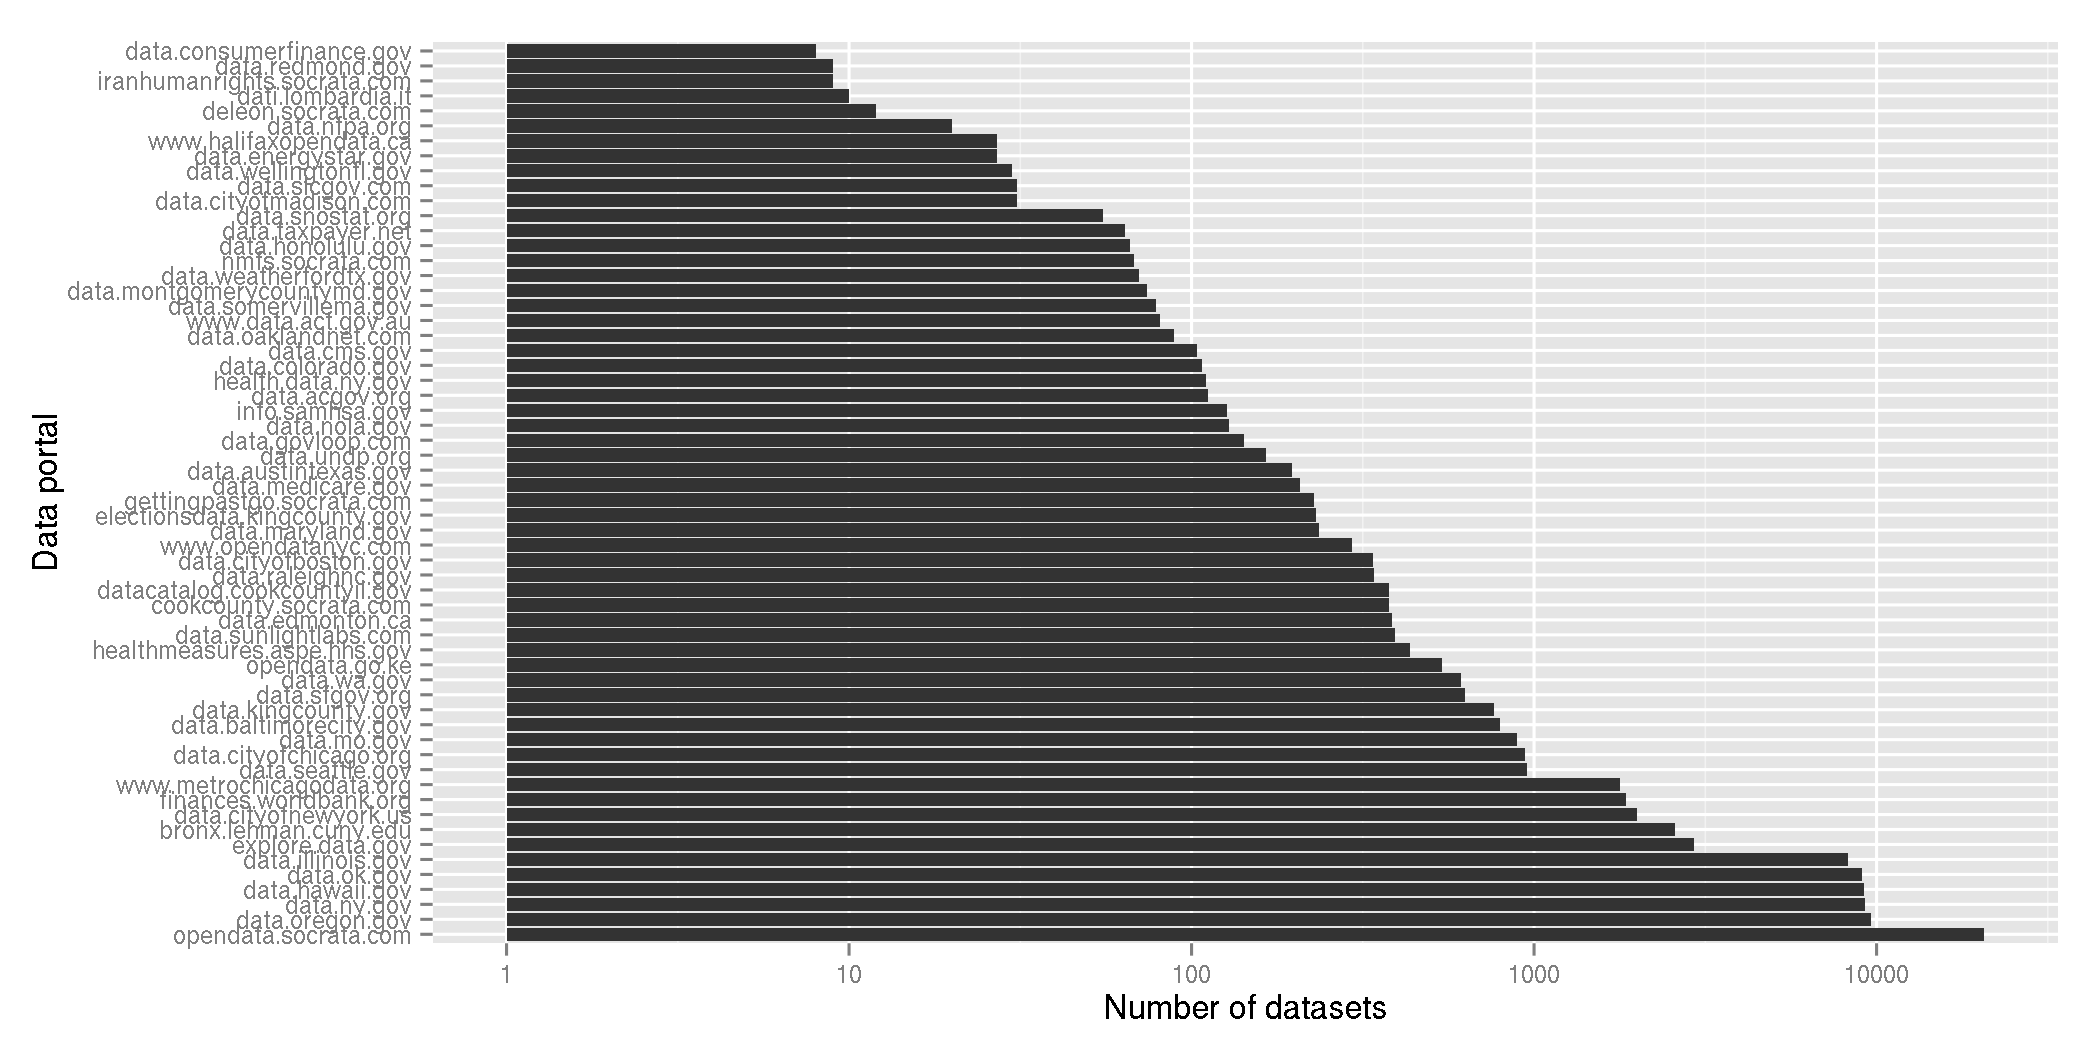
\includegraphics[width=\columnwidth]{../socrata-summary/figure/big_portals_datasets.png}
\caption{How many datasets (spreadsheets) each data catalog had}
\centering
\end{figure}

The smaller sites had just a few spreadsheets, and the larger sites had thousands.

\subsection{Meaninglessness of the count of datasets} \label{colnames}
Many organizations report this count of datasets that they publish, and this number
turns out to be nearly useless. As illustration of this, let's consider a specific
group of spreadsheets. Here are the titles of a few spreadsheets in New York City's
open data catalog.

\begin{itemize}
\item Math Test Results 2006-2012 - Citywide - Gender
\item Math Test Results 2006-2012 - Citywide - Ethnicity
\item English Language Arts (ELA) Test Results 2006-2012 - Citywide - SWD
\item English Language Arts (ELA) Test Results 2006-2012 - Citywide - ELL
\item Math Test Results 2006-2012 - Citywide - SWD
\item English Language Arts (ELA) Test Results 2006-2012 - Citywide - All Students
\item Math Test Results 2006-2012 - Citywide - ELL
\item English Language Arts (ELA) Test Results 2006-2012 - Citywide - Gender
\item Math Test Results 2006-2012 - Citywide - All Students
\item English Language Arts (ELA) Test Results 2006-2012 - Citywide - Ethnicity
\end{itemize}

These spreadsheets all had the same column names; they were

\begin{itemize}
\item grade
\item year
\item demographic
\item number\_tested
\item mean\_scale\_score
\item num\_level\_1
\item pct\_level\_1
\item num\_level\_2
\item pct\_level\_2
\item num\_level\_3
\item pct\_level\_3
\item num\_level\_4
\item pct\_level\_4
\item num\_level\_3\_and\_4
\item pct\_level\_3\_and\_4
\end{itemize}

These "datasets" can all be thought of as subsets of the same single dataset.
If I just take different subsets of a single spreadsheet (and optionally
pivot/reshape the subsets), I can easily expand one spreadsheet into over 9000.
This is why the dataset count figure is near useless.

\subsection{Size of the datasets}
I can also look at how big they are.
It turns out that most of them are pretty small.

\begin{itemize}
\item Only 25% of datasets had more than 100 rows.
\item Only 12% of datasets had more than 1,000 rows.
\item Only 5% of datasets had more than 10,000 rows.
\end{itemize}

%   s <- read.csv('~/t/socrata-analysis/socrata-deduplicated.csv')
%   sum(is.na(s$nrow))                                                                                                  
% [1] 476
%   mean(s$nrow > 100, na.rm = T)                                                                                       
% [1] 0.2507369
%   mean(s$nrow > 1000, na.rm = T)                                                                                      
% [1] 0.1162797
%   mean(s$nrow > 10000, na.rm = T)                                                                                     
% [1] 0.05230904
%   mean(s$nrow > 100000, na.rm = T)                                                                                    
% [1] 0.01799659

Regardless of the format of these datasets, you can think of them as
spreadsheets without code, where columns are variables and rows are records.

\section{Measuring how well different spreadsheets follow data publishing guidelines}
Having gotten some feel for the contents of these various data catalogs,
I started running some less arbitrary statistics.
As discussed in section \ref{guidelines}, many groups have written guidelines
as to how data should be published.%
\cite{open-data-census,fivestars,sunlight,sebastopol,odi}
I started coming up with measures of adherence to these guidelines and running
them across all of these datasets.

\subsection{Licensing}


\subsection{Liveliness of links}









\section{Searching for spreadsheets}
I remarked that it's very hard to find spreadsheets that are relevant
to a particular analysis unless you already know that the spreadsheet exists.
Major search engines focus on HTML format web pages, and spreadsheet files
are often not indexed at all. The various data catalog software programs
discussed in section \ref{acquire} include a search feature, but this feature
only works within the particular website. For example, I have to go to the
Dutch government's data catalog website in order to search for Dutch data.

To summarize my thoughts about the common means of searching through
spreadsheets, I see two main issues.
The first issue is that the search is localized to datasets that are published
or otherwise managed by a particular entity; it's hard to search for
spreadsheets without first identifying a specific publisher or repository.
The second issue is that the search method is quite naive; these websites are
usually running crude keyword searches.

Having articulated these difficulties in searching for spreadsheets, I started
trying to address them.

\subsection{Searching across publishers}
When I'm looking for spreadsheets, the publishing organization is unlikely
to be my main concern. For example, if I'm interested in data about the
composition of different pesticides, but I don't really care whether the
data were collected by this city government or by that country government.

And that's why I made OpenPrism. This is a disgustingly simple site that
forwards your search query to 100 other sites that house spreadsheets.
Lots of people use it, and this says something about the inconvenience of
having separate search bars for separate websites.

\subsection{Spreadsheets-specific search algorithms}
The other issue is that our search algorithms don't take advantage of all
of the structure that is encoded in a spreadsheet.
I started to address this issue by pulling schema-related features out
of the spreadsheets (section \ref{colnames}).

\subsection{Spreadsheets as input to a search}
Taking this further, I've been thinking
about what it would mean to have a search engine for spreadsheets.

\begin{figure}
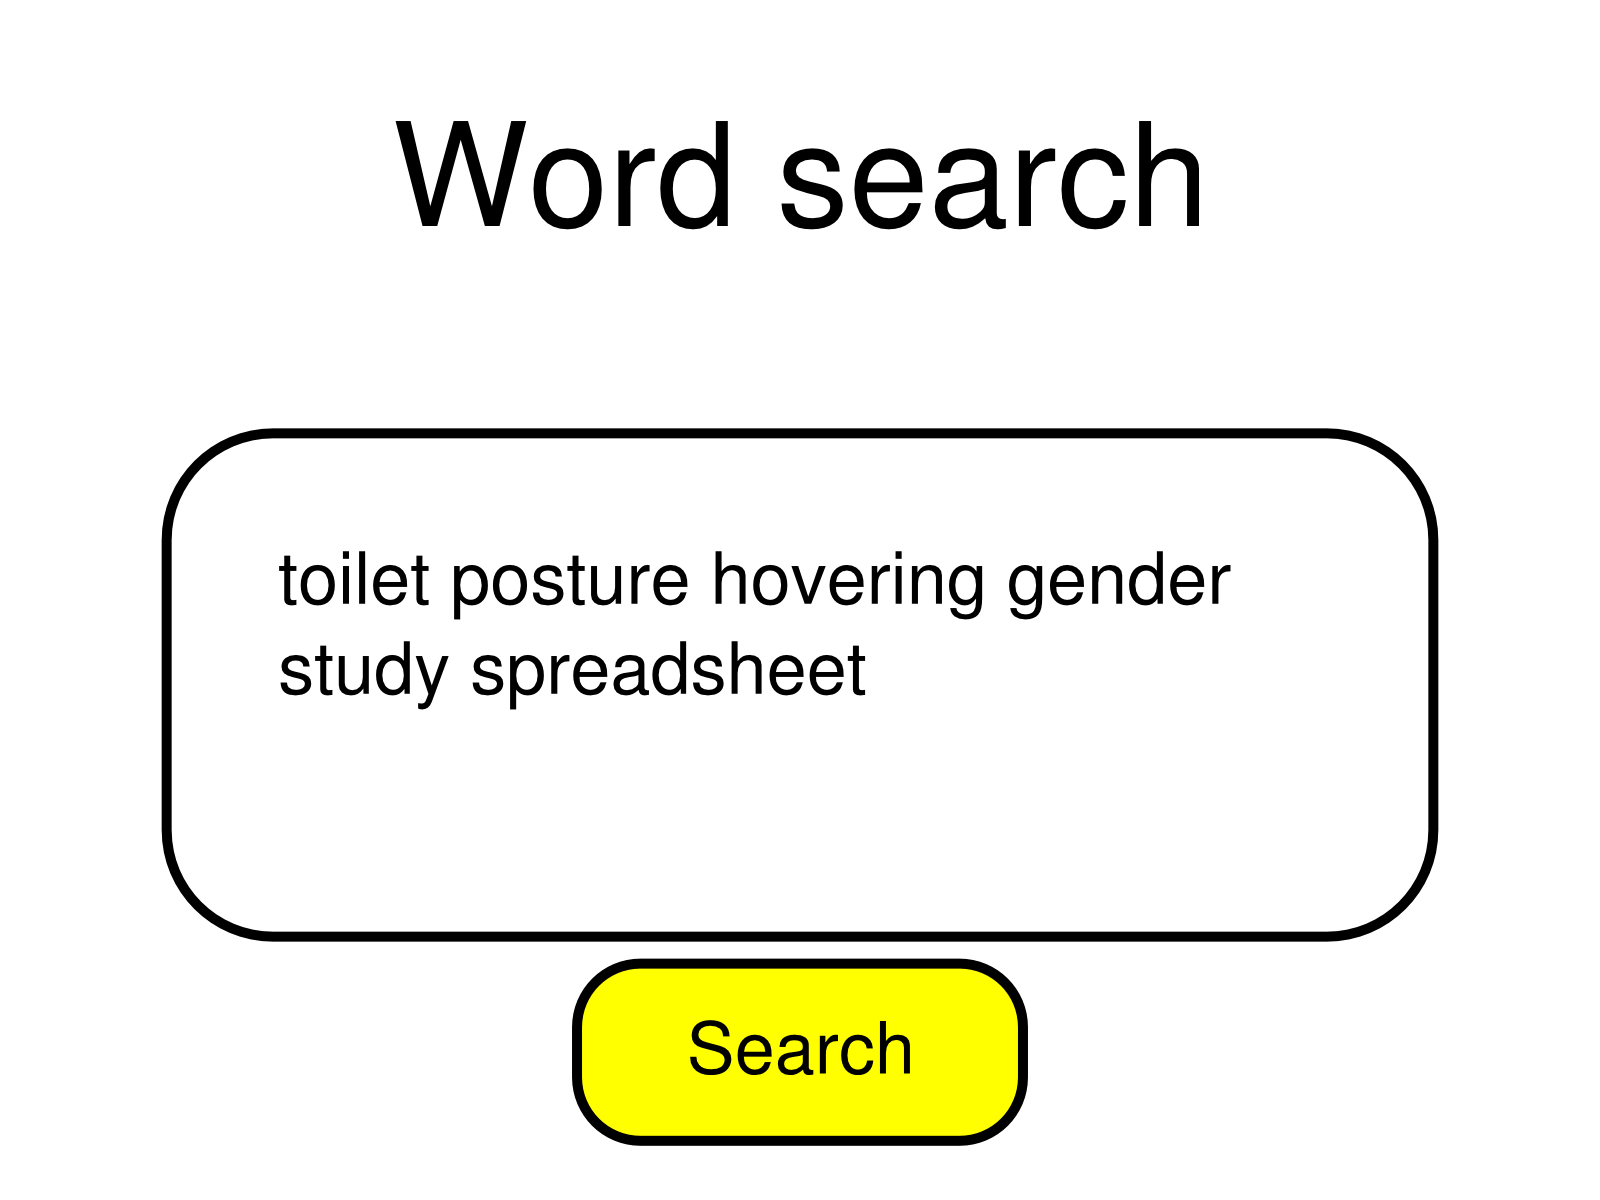
\includegraphics[width=\columnwidth]{../pagerank-for-spreadsheets/wordsearch.png}
\caption{The search engine for words takes words as input and emits words as output}
\centering
\end{figure}

When we search for ordinary written documents, we send words into a search
engine and get pages of words back.

\begin{figure}
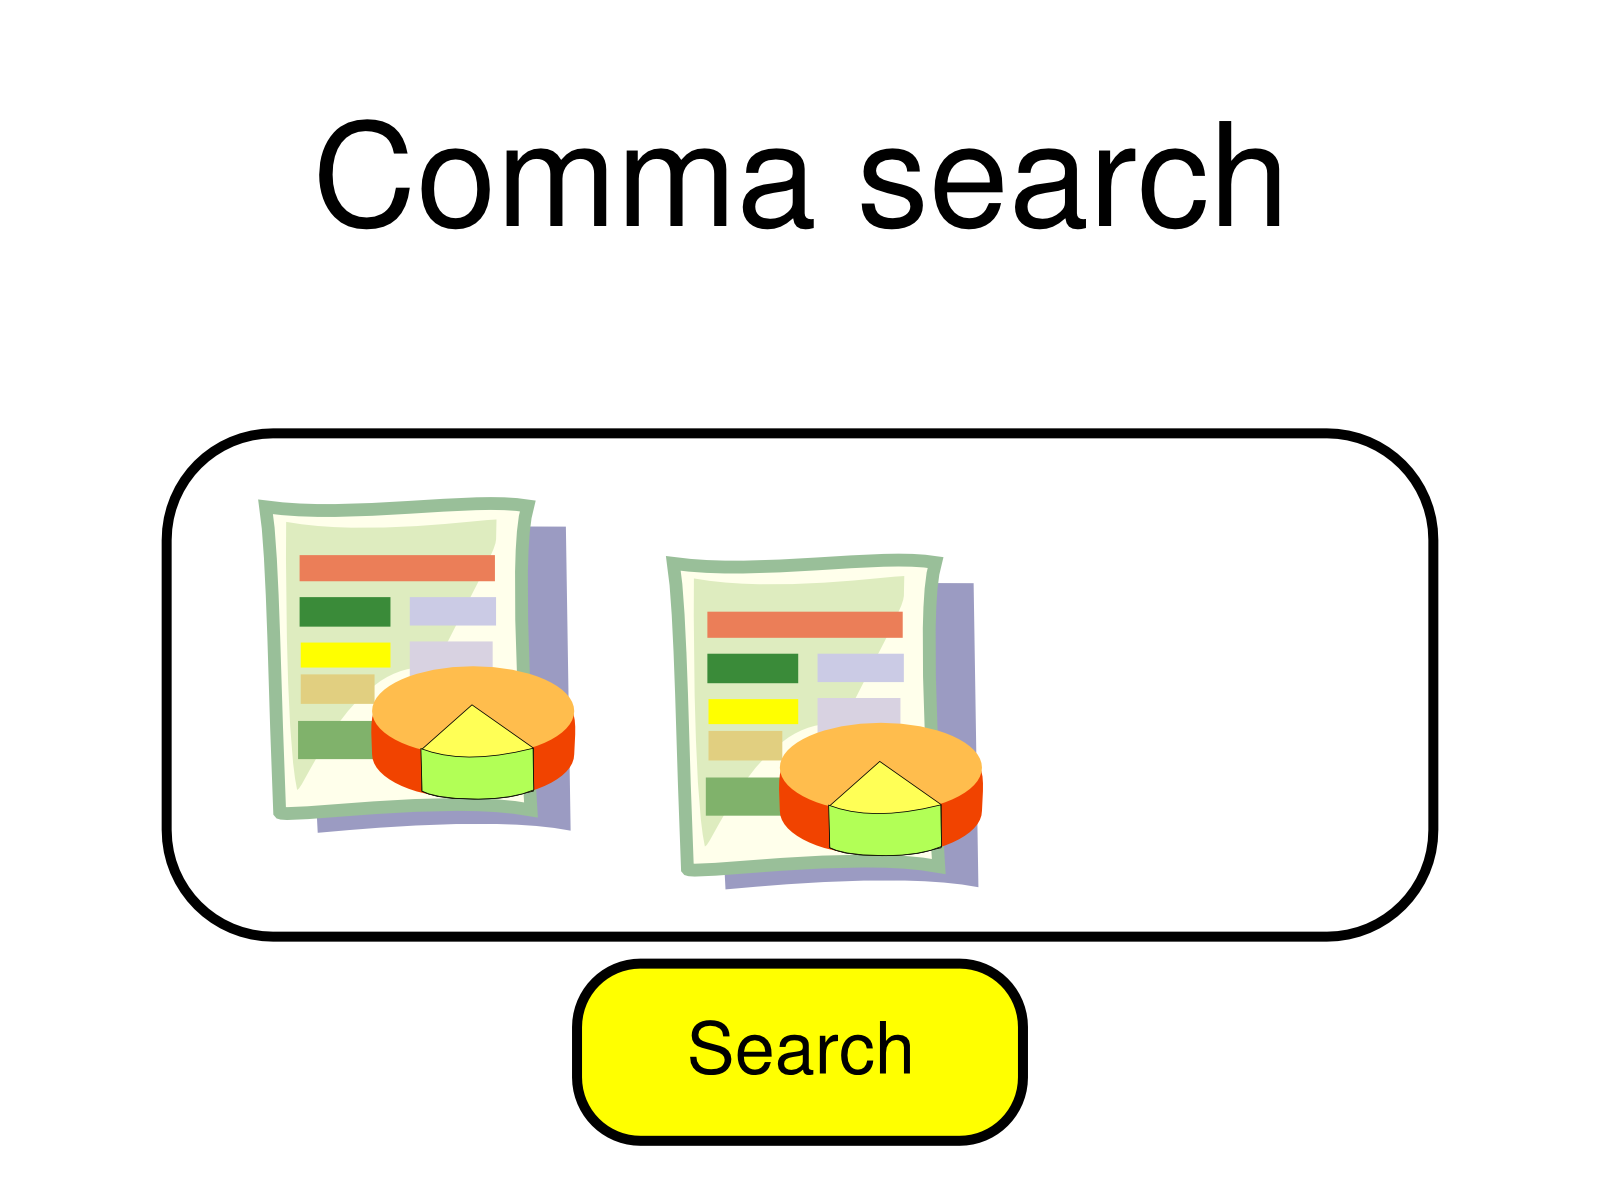
\includegraphics[width=\columnwidth]{../pagerank-for-spreadsheets/commasearch.png}
\caption{The search engine for spreadsheets takes spreadsheets as input and emits spreadsheets as output}
\centering
\end{figure}

What if we could search for spreadsheets
by sending spreadsheets into a search engine and getting spreadsheets back?
The order of the results would be determined by various specialized statistics;
just as we use PageRank to find relevant hypertext documents, we can develop
other statistics that help us find relevant spreadsheets.

\subsubsection{Schema-based searches}
I think a lot about rows and columns. When we define tables in relational
databases, we can say reasonably well what each column means, based on
names and types, and what a row means, based on unique indices.
In spreadsheets, we still have column names, but we don't get everything
else.

The unique indices tell us quite a lot; they give us an idea about the
observational unit of the table and what other tables we can nicely
join or union with that table.

Commasearch \cite{commasearch} is the present state of my spreadsheet search
tools. To use comma search, you first index a lot of spreadsheets. Once you
have the index, you may search by providing a single spreadsheet as input.

In the indexing phase, spreadsheets are examined do find all combinations of
columns that act as unique indices, that is, all combinations of fields whose
values are not duplicated within the spreadsheet. In the search phase,
comma search finds all combinations of columns in the input spreadsheet and
then looks for spreadsheets that are uniquely indexed by these columns.
The results are ordered by how much overlap there is between the values of
the two spreadsheets.

\begin{figure}
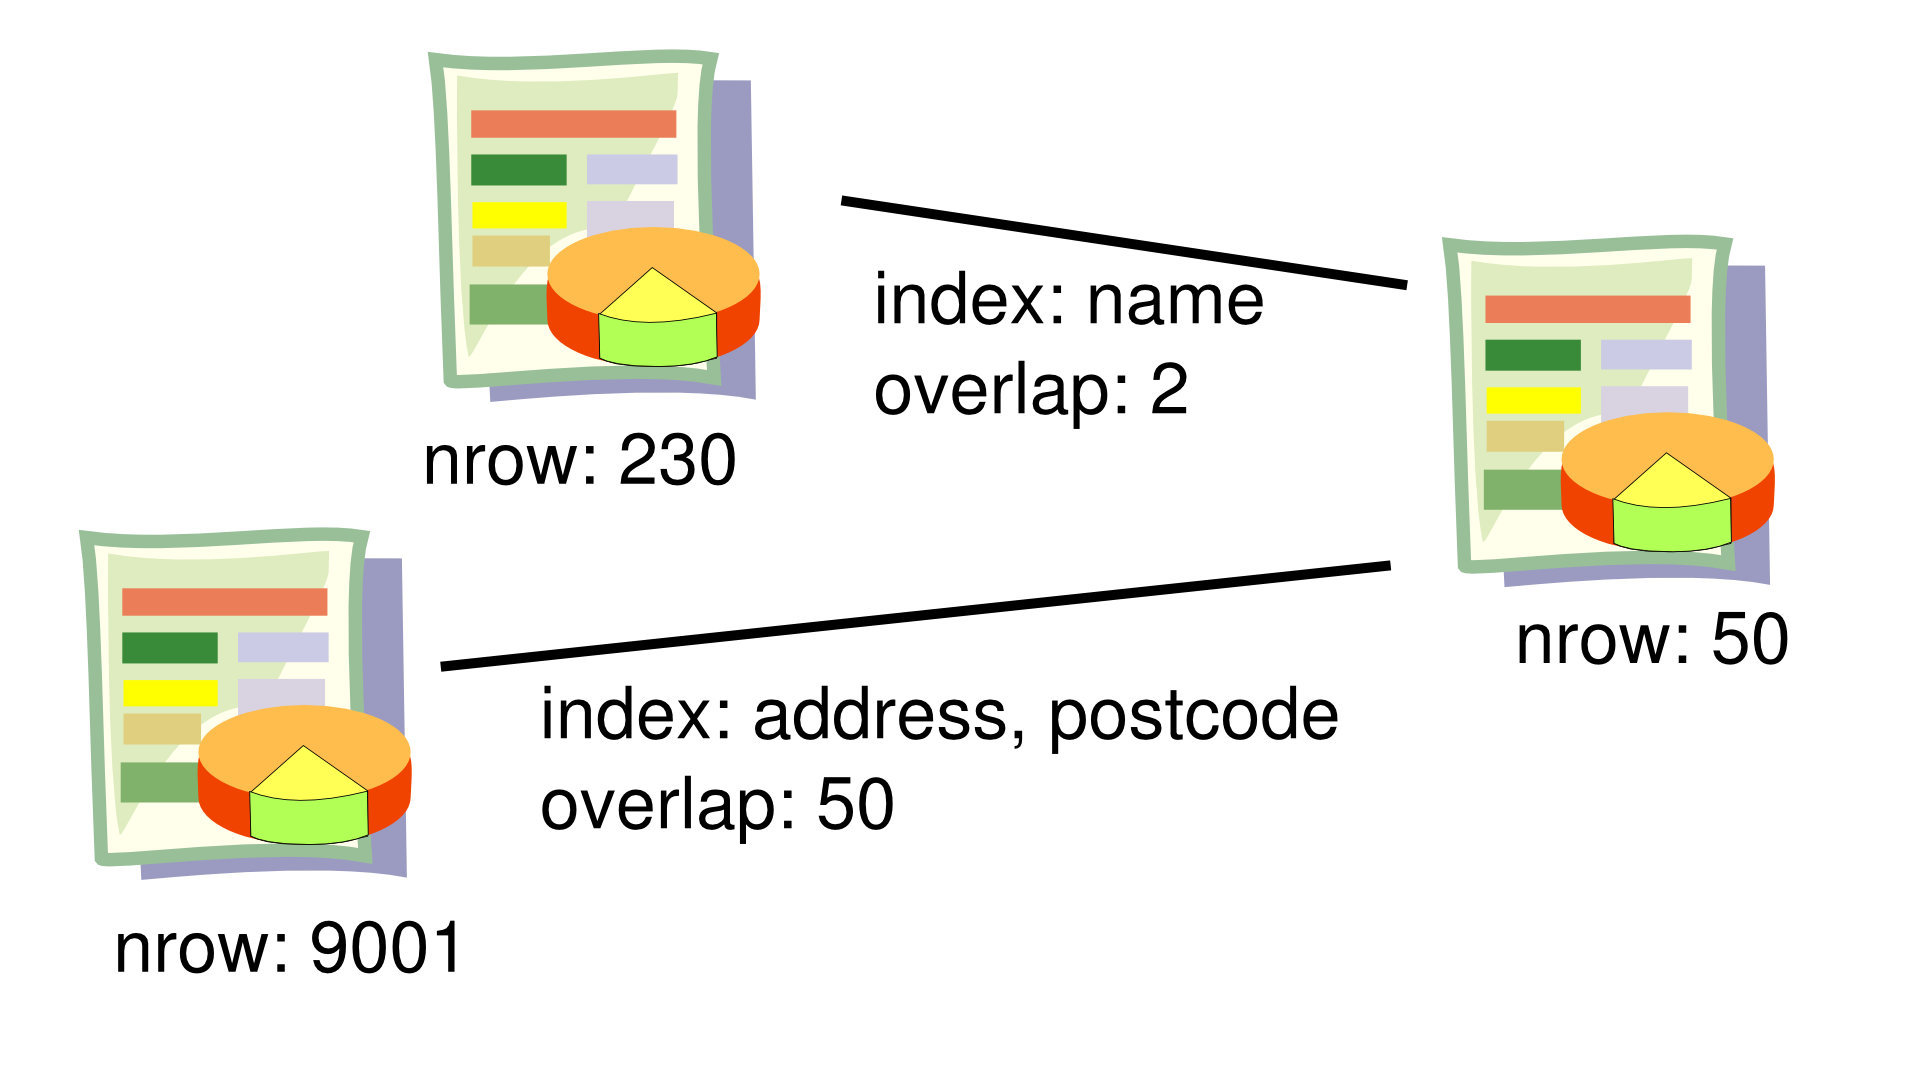
\includegraphics[width=\columnwidth]{../pagerank-for-spreadsheets/network.png}
\caption{Commasearch infers some schema information about each spreadsheet and looks for other spreadsheets with similar schemas.}
\centering
\end{figure}

To say this more colloquially, comma search looks for many-to-one join
relationships between disparate datasets.

\section{Review}
I've been downloading lots of spreadsheets and doing crude, silly things
with them.
I started out by looking at very simple things like how big they are.
I also tried to quantify other people's ideas of how good datasets are,
like whether they are freely licensed. In doing this, I have noticed that
it's pretty hard to search for spreadsheets.

The first issue in search is that you need to type your search into multiple search
bars. Dedicated search engines like DuckDuckGo don't index all of the
spreadsheets, so you're stuck using site-specific searches, and these only
search within their specific sites.

The other issue is that our methods for searching spreadsheets are quite naive.
Most of these data catalogs look for exact string matches in the datasets or
for something similarly crude.

The way we look up information today is to type some words into a search engine
and read the first few results. Why is that not the way we look up data?














\section{Applications}
A couple of people can share a few spreadsheets without any special means,
but it gets hard when there are more than a couple people sharing more than
a few spreadsheets.

Statistics about adherence to data publishing guidelines
can be helpful to those who are tasked
with cataloging and maintaining a diverse array of datasets. Data quality
statistics can provide a quick and timely summary of the issues with different
datasets and allow for a more targeted approach in the maintenance of a
data catalog.

New strategies for searching spreadsheets can help us find data that are
relevant to a topic within the context of analysis.

\bibliographystyle{abbrv}
\bibliography{spreadsheets}
\balancecolumns
\end{document}
